\documentclass{beamer}

\usepackage[spanish]{babel}
\usepackage[utf8]{inputenc}
\usepackage[T1]{fontenc}
\usepackage{amsmath,amssymb,amsfonts}
\usepackage{xcolor}
\usepackage{ragged2e}
\usepackage{etoolbox}
\usepackage{lipsum}
\usepackage{csquotes}
\usepackage[center]{caption}
\usepackage[export]{adjustbox}
\usepackage[backend=biber]{biblatex}

\graphicspath{{../Imágenes}}
\addbibresource{biblio.bib}

\usetheme{Madrid}
\title[Difracción de rayos X]{Difracción de rayos X} 
\author{Luis Lucas García}
\institute[UA]{Universidad de Alicante - Facultad de Ciencias - Grado en física - Ciencia de Materiales}
\date{Mayo de 2025}

\apptocmd{\frame}{}{\justifying}{}
\addtobeamertemplate{block begin}{}{\justifying} % Justify all blocks
\begin{document}
\maketitle
\begin{frame}{Índice}
    \tableofcontents
\end{frame}
\begin{frame}{Difracción \cite{simon2013oxford}}
    \section{Fundamentos teóricos}
    \begin{figure}[h!]
        \begin{center}
            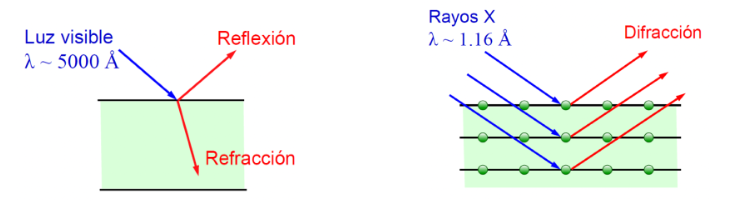
\includegraphics[max width=\linewidth]{Difracciones.png}
        \end{center}
        \caption{Figura de distintas difracciones, para el caso de luz visible y de rayos X.}
    \end{figure}
    Cuando la longitud de onda es comparable a las distancias interatómicas, una gran cantidad de planos contribuye al haz difractado.

    En la mayoría de casos, las interferencias son destructivas. Pero en determinadas direcciones las ondas están en fase y dan lugar al diagrama de difracción.
\end{frame}
\begin{frame}{Ley de Bragg}
    \begin{figure}[h!]
        \begin{center}
            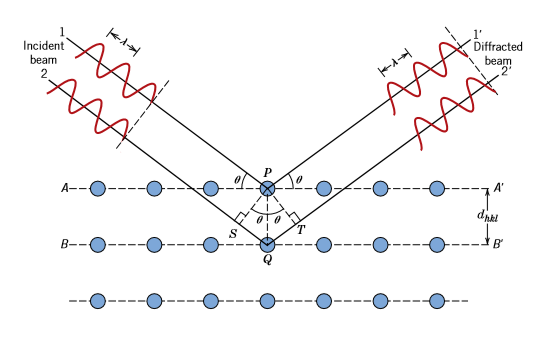
\includegraphics[max width=0.35\linewidth]{BraggLaw.png}
        \end{center}
        \caption{Diagrama de las ondas reflejándose en los planos paralelos del cristal. Figura obtenida de \cite{braggFigure}.}
    \end{figure}
    \begin{block}{Ley de Bragg}
        Bragg supone que las ondas incidentes se reflejan en los planos paralelos del cristal. Para que la difracción sea constructiva debe cumplirse la condición de Bragg:
        \begin{equation}
            2d\sin\theta = n\lambda
            \label{eq:braggLaw}
        \end{equation}
    \end{block}
\end{frame}
\begin{frame}{Amplitudes de Scattering}
    En el espacio recíproco existe la ley de Laue, que nos exige que $|\vec{k}| = |\vec{k}'| = \frac{2\pi}{\lambda}$, donde $\vec{k}'$ es el vector de onda tras la reflexión y viceversa.
    \begin{block}{Factor de estructura}
        Obtenemos con la regla de oro de Fermi, unos elementos de matriz, en los que el factor de estructura será:
        \begin{equation}
            S(\vec{G}) = \int_{celda \, unidad} d\vec{r} \, e^{-i\vec{G}\cdot\vec{r}}V(\vec{r})
        \end{equation}
        Siendo la intensidad de la difracción, el módulo cuadrado de este factor de estructura para un plano dado.
    \end{block}
    En la expresión anterior, $\vec{G}$, es el vector de la red recíproca, que es la red constituida por la transformada de Fourier al espacio $\vec{k}$ de la red cristalina.
\end{frame}
\begin{frame}{Amplitudes en rayos X}
    \begin{block}{Factor de forma}
        Esta expresión se simplifica en gran medida al considerar difracción por rayos X. Ahora tendremos:
        \begin{equation}
            S(\vec{G}) = \sum_j f_j(\vec{G})e^{i\vec{G}\cdot\vec{x}_j}
         \end{equation}
    \end{block}
    En esta expresión, $f_j$ es el factor de forma que podemos calcular como:
    $$
    f_j(\vec{G}) = \int d\vec{x} \, e^{i\vec{G}\cdot\vec{x}_j}V_j(\vec{x})
    $$
    Se puede considerar modelos simplificados de este factor de forma, como un modelo que lo haga constante o uno de esferas rígidas, que funcionan bien como primeras aproximaciones. En nuestros cálculos no nos preocuparemos de dar el factor de forma, y los tomaremos como constantes.
\end{frame}
\begin{frame}{Estructura de planos}
    \begin{block}{Una última consideración}
        Si consideramos los ejes ortogonales (caso de una red cúbica), y además el parámetro de red idéntico en las tres direcciones, podemos relacionar el parámetro de red con la distancia interplanar tal que:
        \begin{equation}
            d_{(hkl)}^2 = \frac{a^2}{h^2 + k^2 + l^2}
            \label{eq:lattParam}
        \end{equation}
    \end{block}
    \begin{figure}[h!]
        \begin{center}
            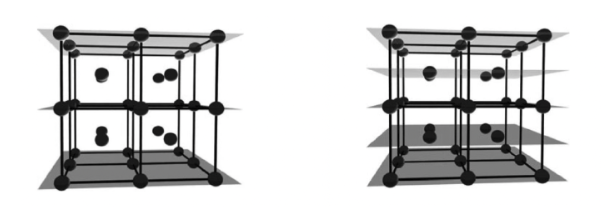
\includegraphics[max width=0.65\linewidth]{planosEstadoSolido.png}
        \end{center}
        \caption{Imagen de las familias de planos (010) y (020) en una red BCC. Imagen tomada de las diapositivas de física del estado sólido - prof. Carlos Untiedt.}
    \end{figure}
\end{frame}
\begin{frame}{La estructura del $NaCl$}
    \subsection{Estructura de la sal}
    En la imagen podemos observar que el cloruro de sodio consta de una base con dos átomos, uno de ellos centrado en $(0, 0, 0)$ y el otro en $\left(\frac{1}{2}, \frac{1}{2}, \frac{1}{2}\right)$, ambos ocupando las posiciones de una red FCC.
    \begin{figure}[h!]
        \begin{center}
            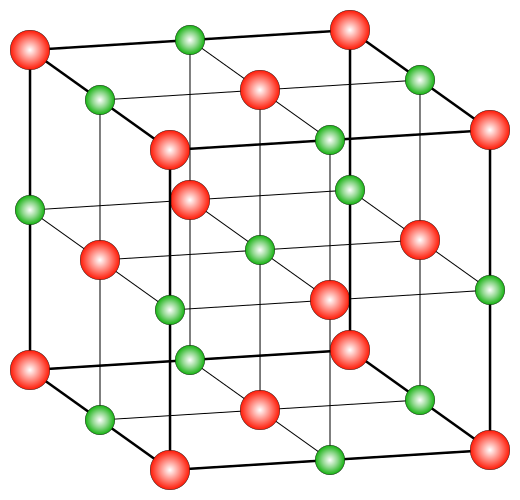
\includegraphics[max width=0.35\linewidth]{Ionlattice-fcc.svg.png}
        \end{center}
        \caption{Imagen de la estructura del $NaCl$, obtenida de Wikimedia del usuario Prolineserver en el siguiente enlace: \href{https://commons.wikimedia.org/wiki/File:Ionlattice-fcc.svg}{[ENLACE]}}
    \end{figure}
\end{frame}
\begin{frame}{Amplitud de difracción de la sal}
    \subsection{Amplitud de difracción de la sal}
    Podemos obtener la amplitud de la difracción. Multiplicamos la parte asociada a la base de la debida a los vectores de la red:
    \begin{equation}
        S_{(hkl)} = \left(f_{Na} + f_{Cl}e^{i\pi(h+k+l)}\right)\left(1 + e^{i\pi(h+k)} + e^{i\pi(h+l)} + e^{i\pi(k+l)}\right)
    \end{equation}
    Esta expresión nos permite obtener en primera aproximación y de un vistazo las condiciones de extinción.
    \begin{block}{Condiciones de extinción}
        \begin{itemize}
            \item La amplitud de scattering se cancela, salvo que $h$, $k$ y $l$ sean los tres pares o impares. Es decir, aparecen picos en $(111)$, $(200)$, etc.
            \item En el caso de que todos los picos sean impares, observaremos un mínimo pues en la parte de base tendremos $f_{Na} - f_{Cl}$, mientras que en el caso de todos pares tendremos un pico más alto: $f_{Na} + f_{Cl}$.
        \end{itemize}
    \end{block}
\end{frame}
\begin{frame}{Dispositivo experimental}
    \section{Desarrollo}
    \subsection{Obtención de rayos X}
    \begin{figure}[h!]
        \begin{center}
            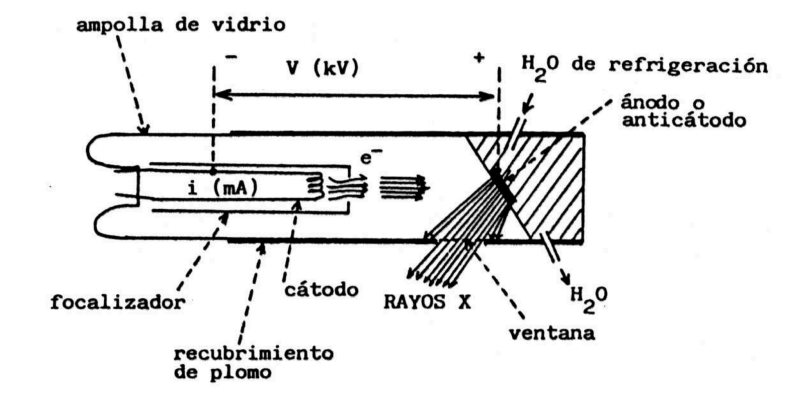
\includegraphics[max width=0.95\linewidth]{xRayDevice.png}
        \end{center}
        \caption{Esquema de un tubo de rayos X de cátodo incandescente. Imagen obtenida del propio guión de las prácticas.}
    \end{figure}
\end{frame}
\begin{frame}{Preparación de la muestra y obtención del patrón}
    \subsection{Preparación de la muestra y obtención del patrón}
    \begin{block}{Preparación de la muestra}
        Vamos a moler la muestra cristalina hasta obtener un polvo fino homogéneo. De esta manera, los pequeños cristales estarán orientados en todas las direcciones, de forma que la difracción no favorezca a ningún plano.
    \end{block}
    \begin{block}{Obtención del patrón}
        Para obtener el patrón, hacemos girar la fuente de rayos X para hacerlos incidir en distintos ángulos. Mediremos la intensidad de los rayos difractados respecto al ángulo doble, $2\theta$.
    \end{block}
    \begin{figure}[h!]
        \begin{center}
            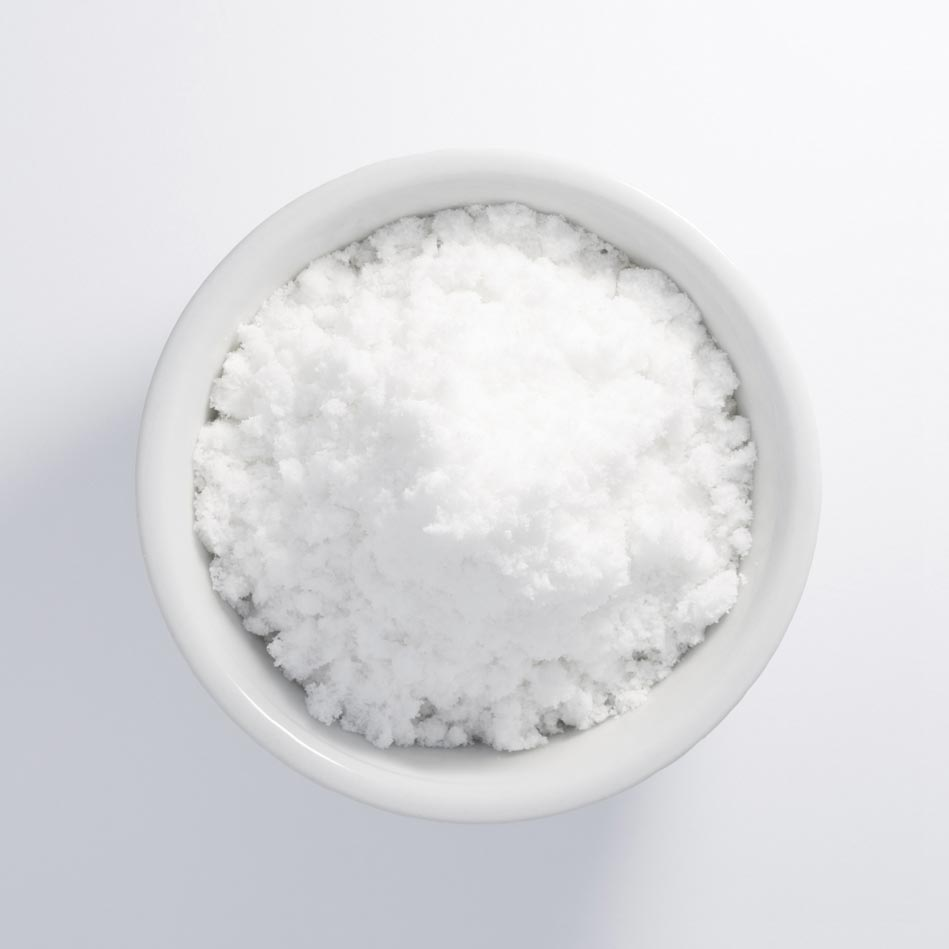
\includegraphics[max width=0.12\linewidth]{Salinera-Espanola_Muestra-Sal-polvo.jpg}
        \end{center}
        \caption{Sal comercial en polvo. La de nuestra muestra debería ser aún más fina y estar esparcida en una fina capa sobre un portamuestras.}
    \end{figure}
\end{frame}
\begin{frame}{Resultados}
    \section{Resultados}
    \begin{figure}[h!]
        \begin{center}
            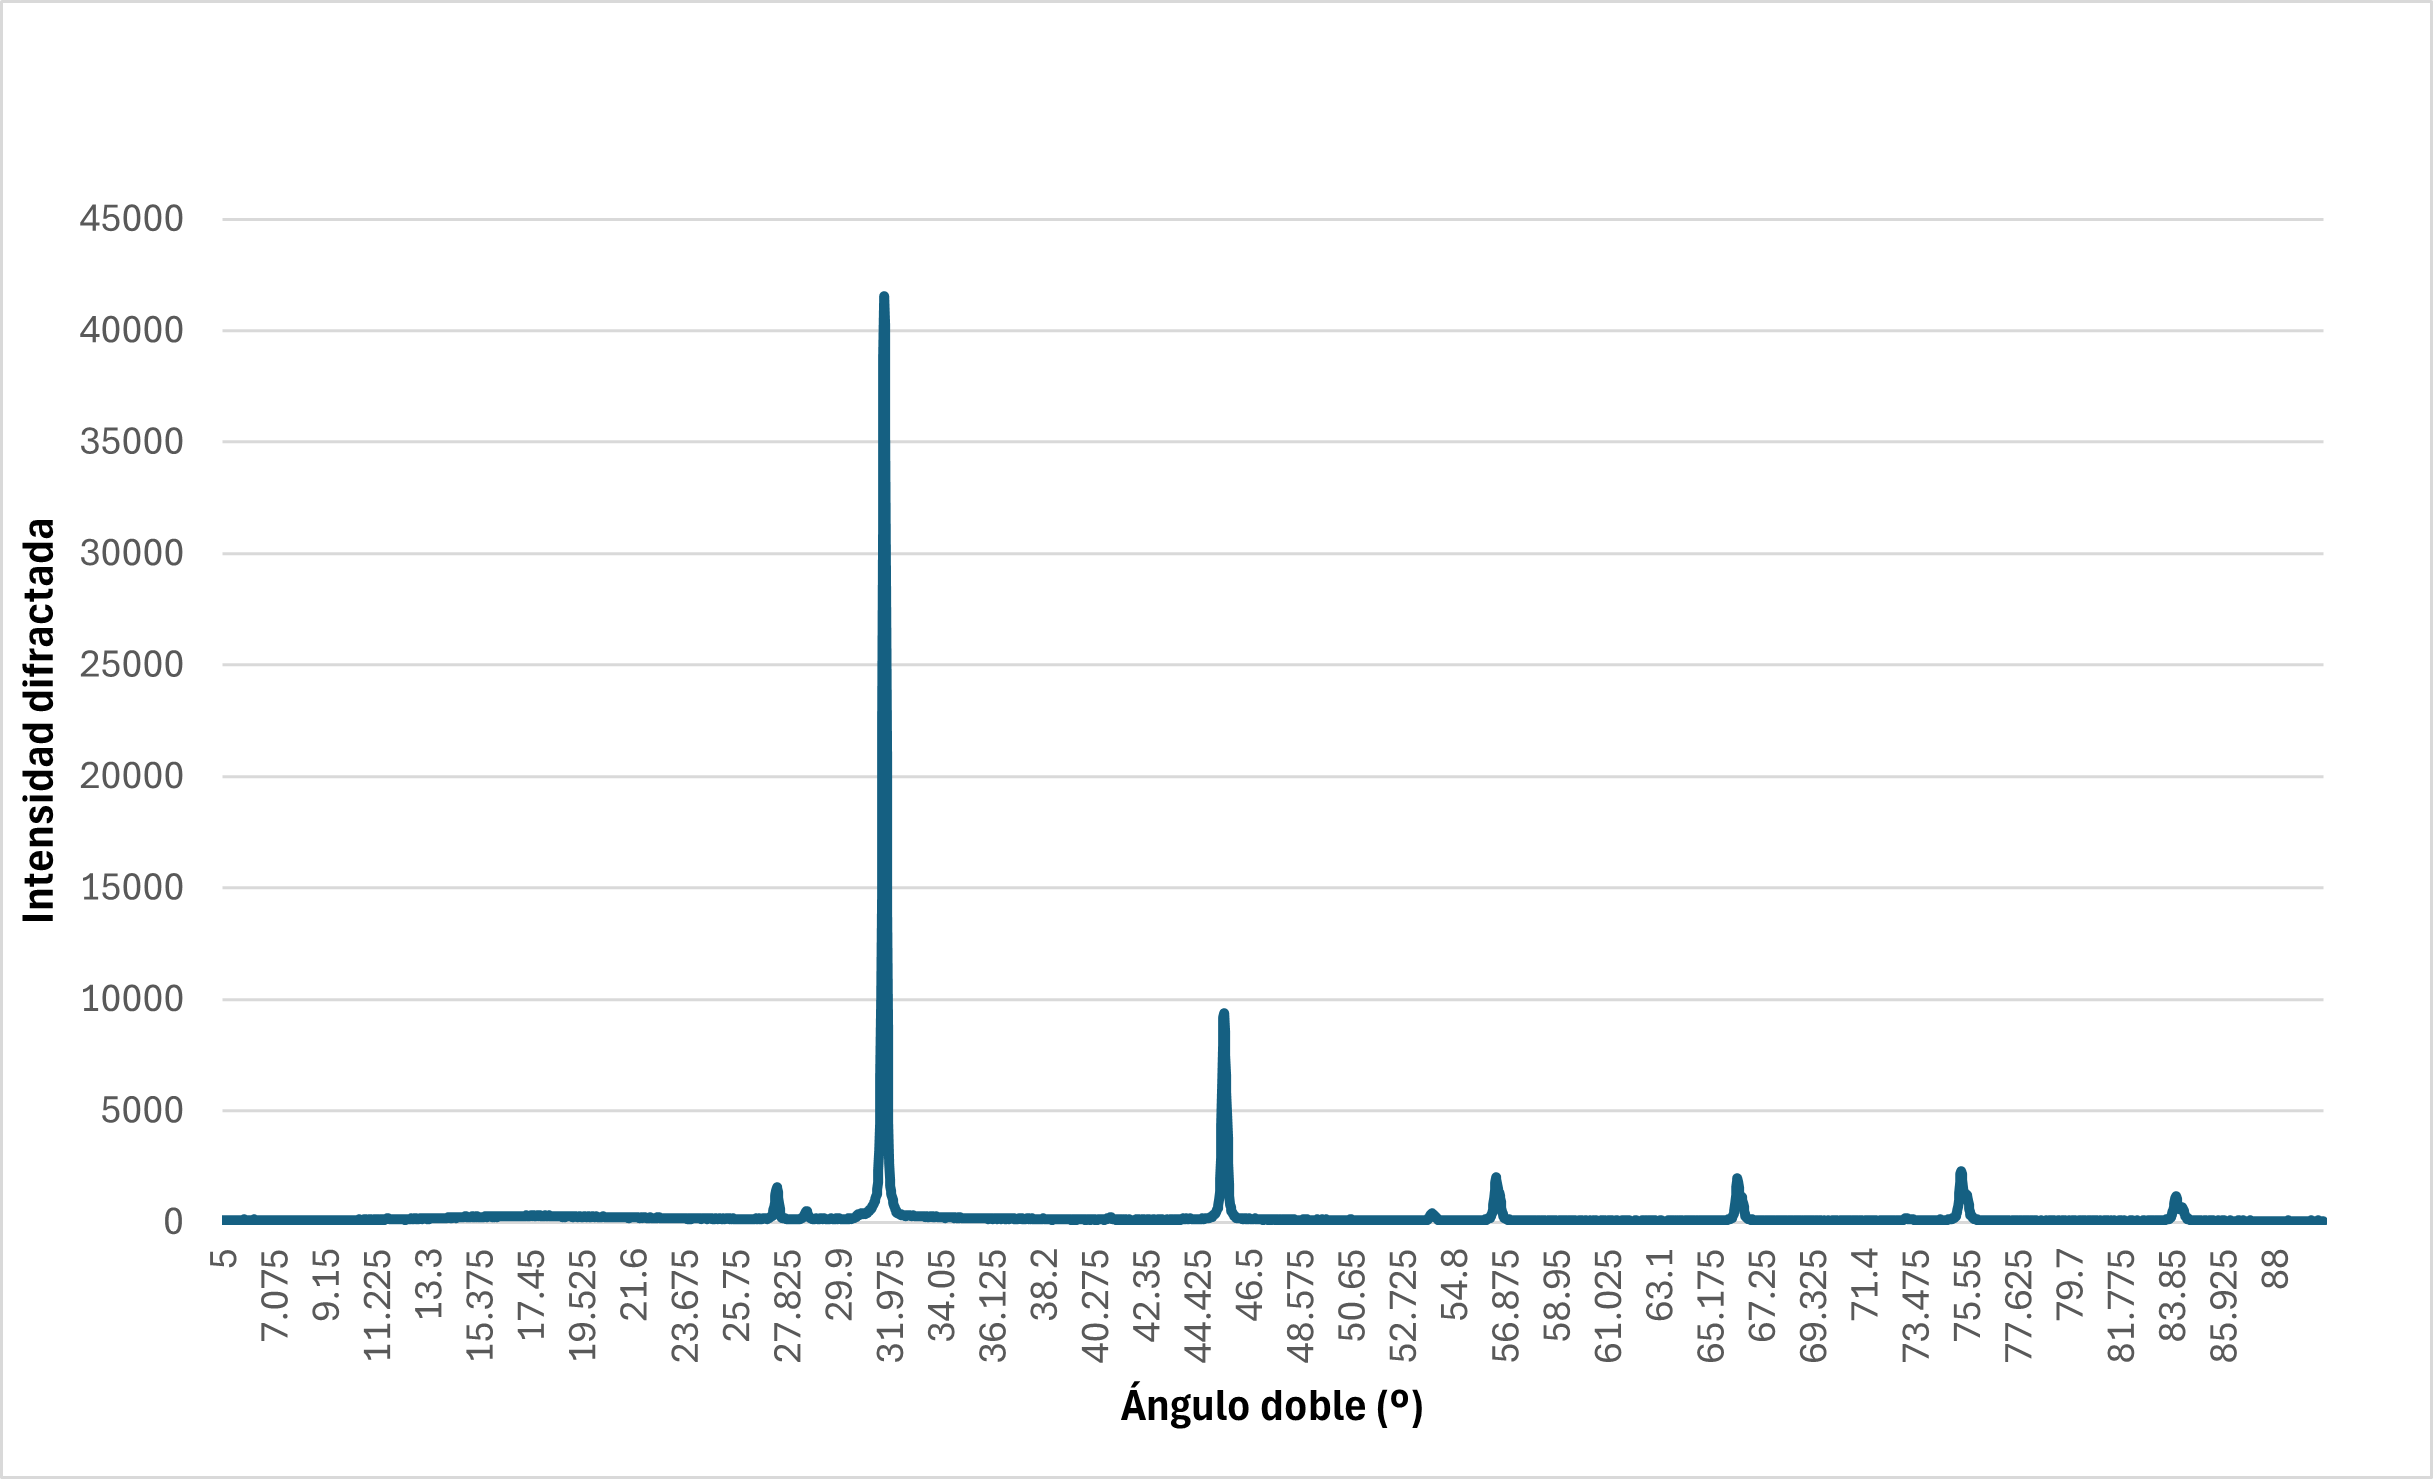
\includegraphics[max width=0.9\linewidth]{DifNaCl.png}
        \end{center}
        \caption{Picos de difracción obtenidos para el cloruro de sodio.}
    \end{figure}
\end{frame}
\begin{frame}{Distancias interplanares}
    \subsection{Distancias entre planos}
    Usando la ley de Bragg, podemos calcular las distancias entre planos para los tres primeros picos. Sabiendo que la longitud de onda es de $\lambda = 0.1541nm$
    \begin{table}
        \begin{center}
            \begin{tabular}{|c|c|c|c|c|c|}
                \hline
                d (\r{A}) & $2.815$ & $1.991$ & $1.699$ & $3.250$ & $1.627$ \\ \hline
                $2\theta$ (º) & $31.775$ & $45.525$ & $53.925$ & $27.425$ & $56.525$ \\ \hline
            \end{tabular}
        \end{center}
        \caption{Tabla de distancias interplanares obtenidas para varios ángulos.}
    \end{table}
    \begin{figure}[h!]
        \begin{center}
            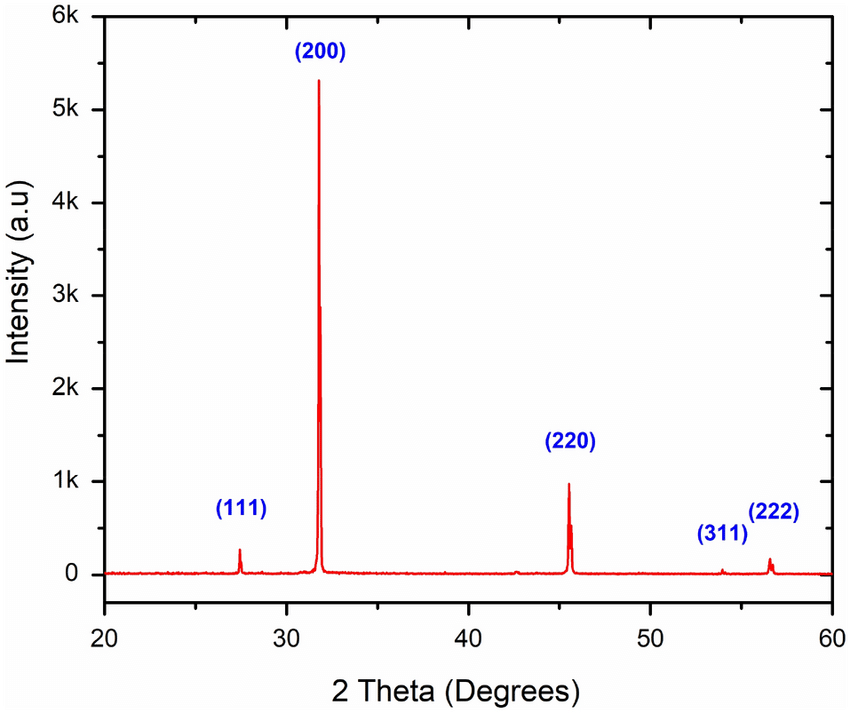
\includegraphics[max width=0.35\linewidth]{DifArticle.png}
        \end{center}
        \caption{Imagen de difracción de rayos X para la sal tomada de la referencia \cite{difArticle}.}
    \end{figure}
\end{frame}
\begin{frame}
    Usando la referencia \cite{difArticle}, podemos asignar a cada uno de los picos anteriores un plano:
    \begin{table}
        \begin{center}
            \begin{tabular}{|c|c|c|c|c|c|}
                \hline
                (hkl) & (200) & (220) & (311) & (111) & (222) \\ \hline
                d (\r{A}) & $2.815$ & $1.991$ & $1.699$ & $3.250$ & $1.627$ \\ \hline
                $2\theta$ (º) & $31.775$ & $45.525$ & $53.925$ & $27.425$ & $56.525$ \\ \hline
            \end{tabular}
        \end{center}
        \caption{Tabla de distancias interplanares obtenidas para varios ángulos con los correspondientes índices de los planos a los que pertenecen.}
    \end{table}
    \begin{figure}[h!]
        \begin{center}
            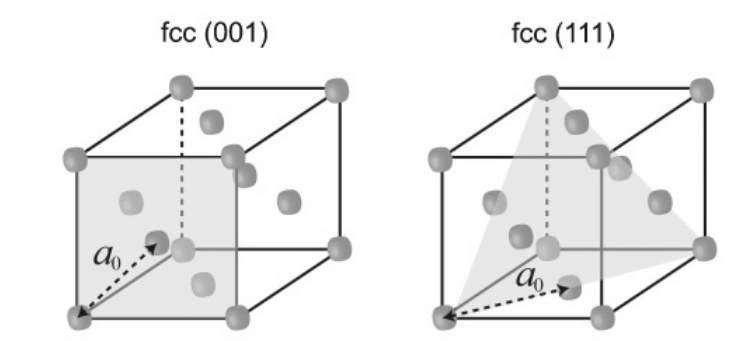
\includegraphics[max width=0.6\linewidth]{planosFCC.png}
        \end{center}
        \caption{Algunos planos de estructuras FCC. Fragmento de imagen tomado de la referencia \cite{fccPlanes}.}
    \end{figure}
\end{frame}
\begin{frame}{Parámetro de red}
    \subsection{Parámetro de red}
    Usemos ahora la ecuación \ref{eq:lattParam}, nos permitirá obtener el parámetro de red.
    \begin{table}
        \begin{center}
            \begin{tabular}{|c|c|c|c|c|c|}
                \hline
                (hkl) & (200) & (220) & (311) & (111) & (222) \\ \hline
                d (\r{A}) & $2.815$ & $1.991$ & $1.699$ & $3.250$ & $1.627$ \\ \hline
                $2\theta$ (º) & $31.775$ & $45.525$ & $53.925$ & $27.425$ & $56.525$ \\ \hline
                a (\r{A}) & $5.629$ & $5.633$ & $5.636$ & $5.630$ & $5.637$ \\ \hline
            \end{tabular}
        \end{center}
        \caption{Tabla de distancias interplanares obtenidas para varios ángulos con los correspondientes índices de los planos a los que pertenecen y los parámetros de red obtenidos en cada caso.}
    \end{table}
    \begin{block}{Resultado final}
        Si ahora, promediamos y tomamos como error en la medida la desviación estándar, nuestro valor del parámetro de red es:
        \begin{equation}
            a = 5.633 \pm 0.003 \, \text{\r{A}}
        \end{equation}
    \end{block}
\end{frame}
\begin{frame}{Comparación de resultados}
    \subsection{Comparación de resultados}
    Si queremos conseguir un $99.995\%$ de confianza en la medida, multiplicamos este error siguiendo la tabla t-student, y nos quedaría, con la confianza del $99.995\%$. El error relativo es del $0.21\%$, lo que lo hace una buena medida:
    $$
    a = 5.633 \pm 0.012 \, \text{\r{A}}
    $$
    Este valor coincide con el valor de la bibliografía de $a = 5.6402 \, \text{\r{A}}$ \cite{noauthororeditor2007handbook}.
    \begin{block}{Estructura cristalina}
        Además, el diagrama que obtenemos en difracción de rayos X es compatible con la geometría propuesta: dos redes FCC ocupadas por los iones $Na^+$ y $Cl^-$ desplazadas por un vector $\left(\frac{1}{2}, \frac{1}{2}, \frac{1}{2}\right)$.
    \end{block}
    \begin{figure}[h!]
        \begin{center}
            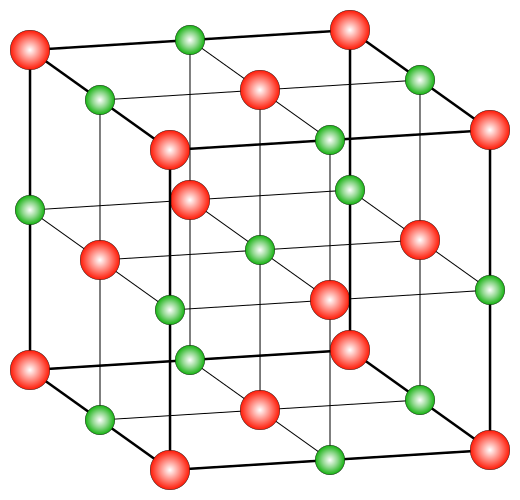
\includegraphics[max width=0.1\linewidth]{Ionlattice-fcc.svg.png}
        \end{center}
        \caption{Imagen de la estructura del $NaCl$, obtenida de Wikimedia del usuario Prolineserver en el siguiente enlace: \href{https://commons.wikimedia.org/wiki/File:Ionlattice-fcc.svg}{[ENLACE]}}
    \end{figure}
\end{frame}
\begin{frame}{Factores de forma}
    \subsection{Factores de forma}
    Podemos intentar calcular de alguna manera los factores de forma, usando que:
    \begin{align*}
    I_{(hkl)} \propto \left|S_{(hkl)}\right|^2 = \\ = \left(f_{Na}^2 + f_{Cl}^2 +2f_{Na}f_{Cl}\cos\left(\pi(h + k + l)\right)\right)*\\ \left(1 + (-1)^{h+k} + (-1)^{h+l} + (-1)^{k+l}\right)^2
    \end{align*}
    Si nos restringimos a los casos en los que no hay extinción, tendremos:
    \begin{itemize}
        \item \textbf{Todos son pares:} en este caso, $I_{(hkl)}^{max} \propto \left(f_{Na} + f_{Cl}\right)^2$.
        \item \textbf{Todos son impares:} en este caso, $I_{(hkl)}^{min} \propto \left(f_{Na} - f_{Cl}\right)^2$.
    \end{itemize}
    El problema es que los diferentes órdenes de difracción van perdiendo intensidad. Tenemos que trabajar con pares de picos e intensidades relativas.
\end{frame}
\begin{frame}
    \begin{figure}[h!]
        \begin{center}
            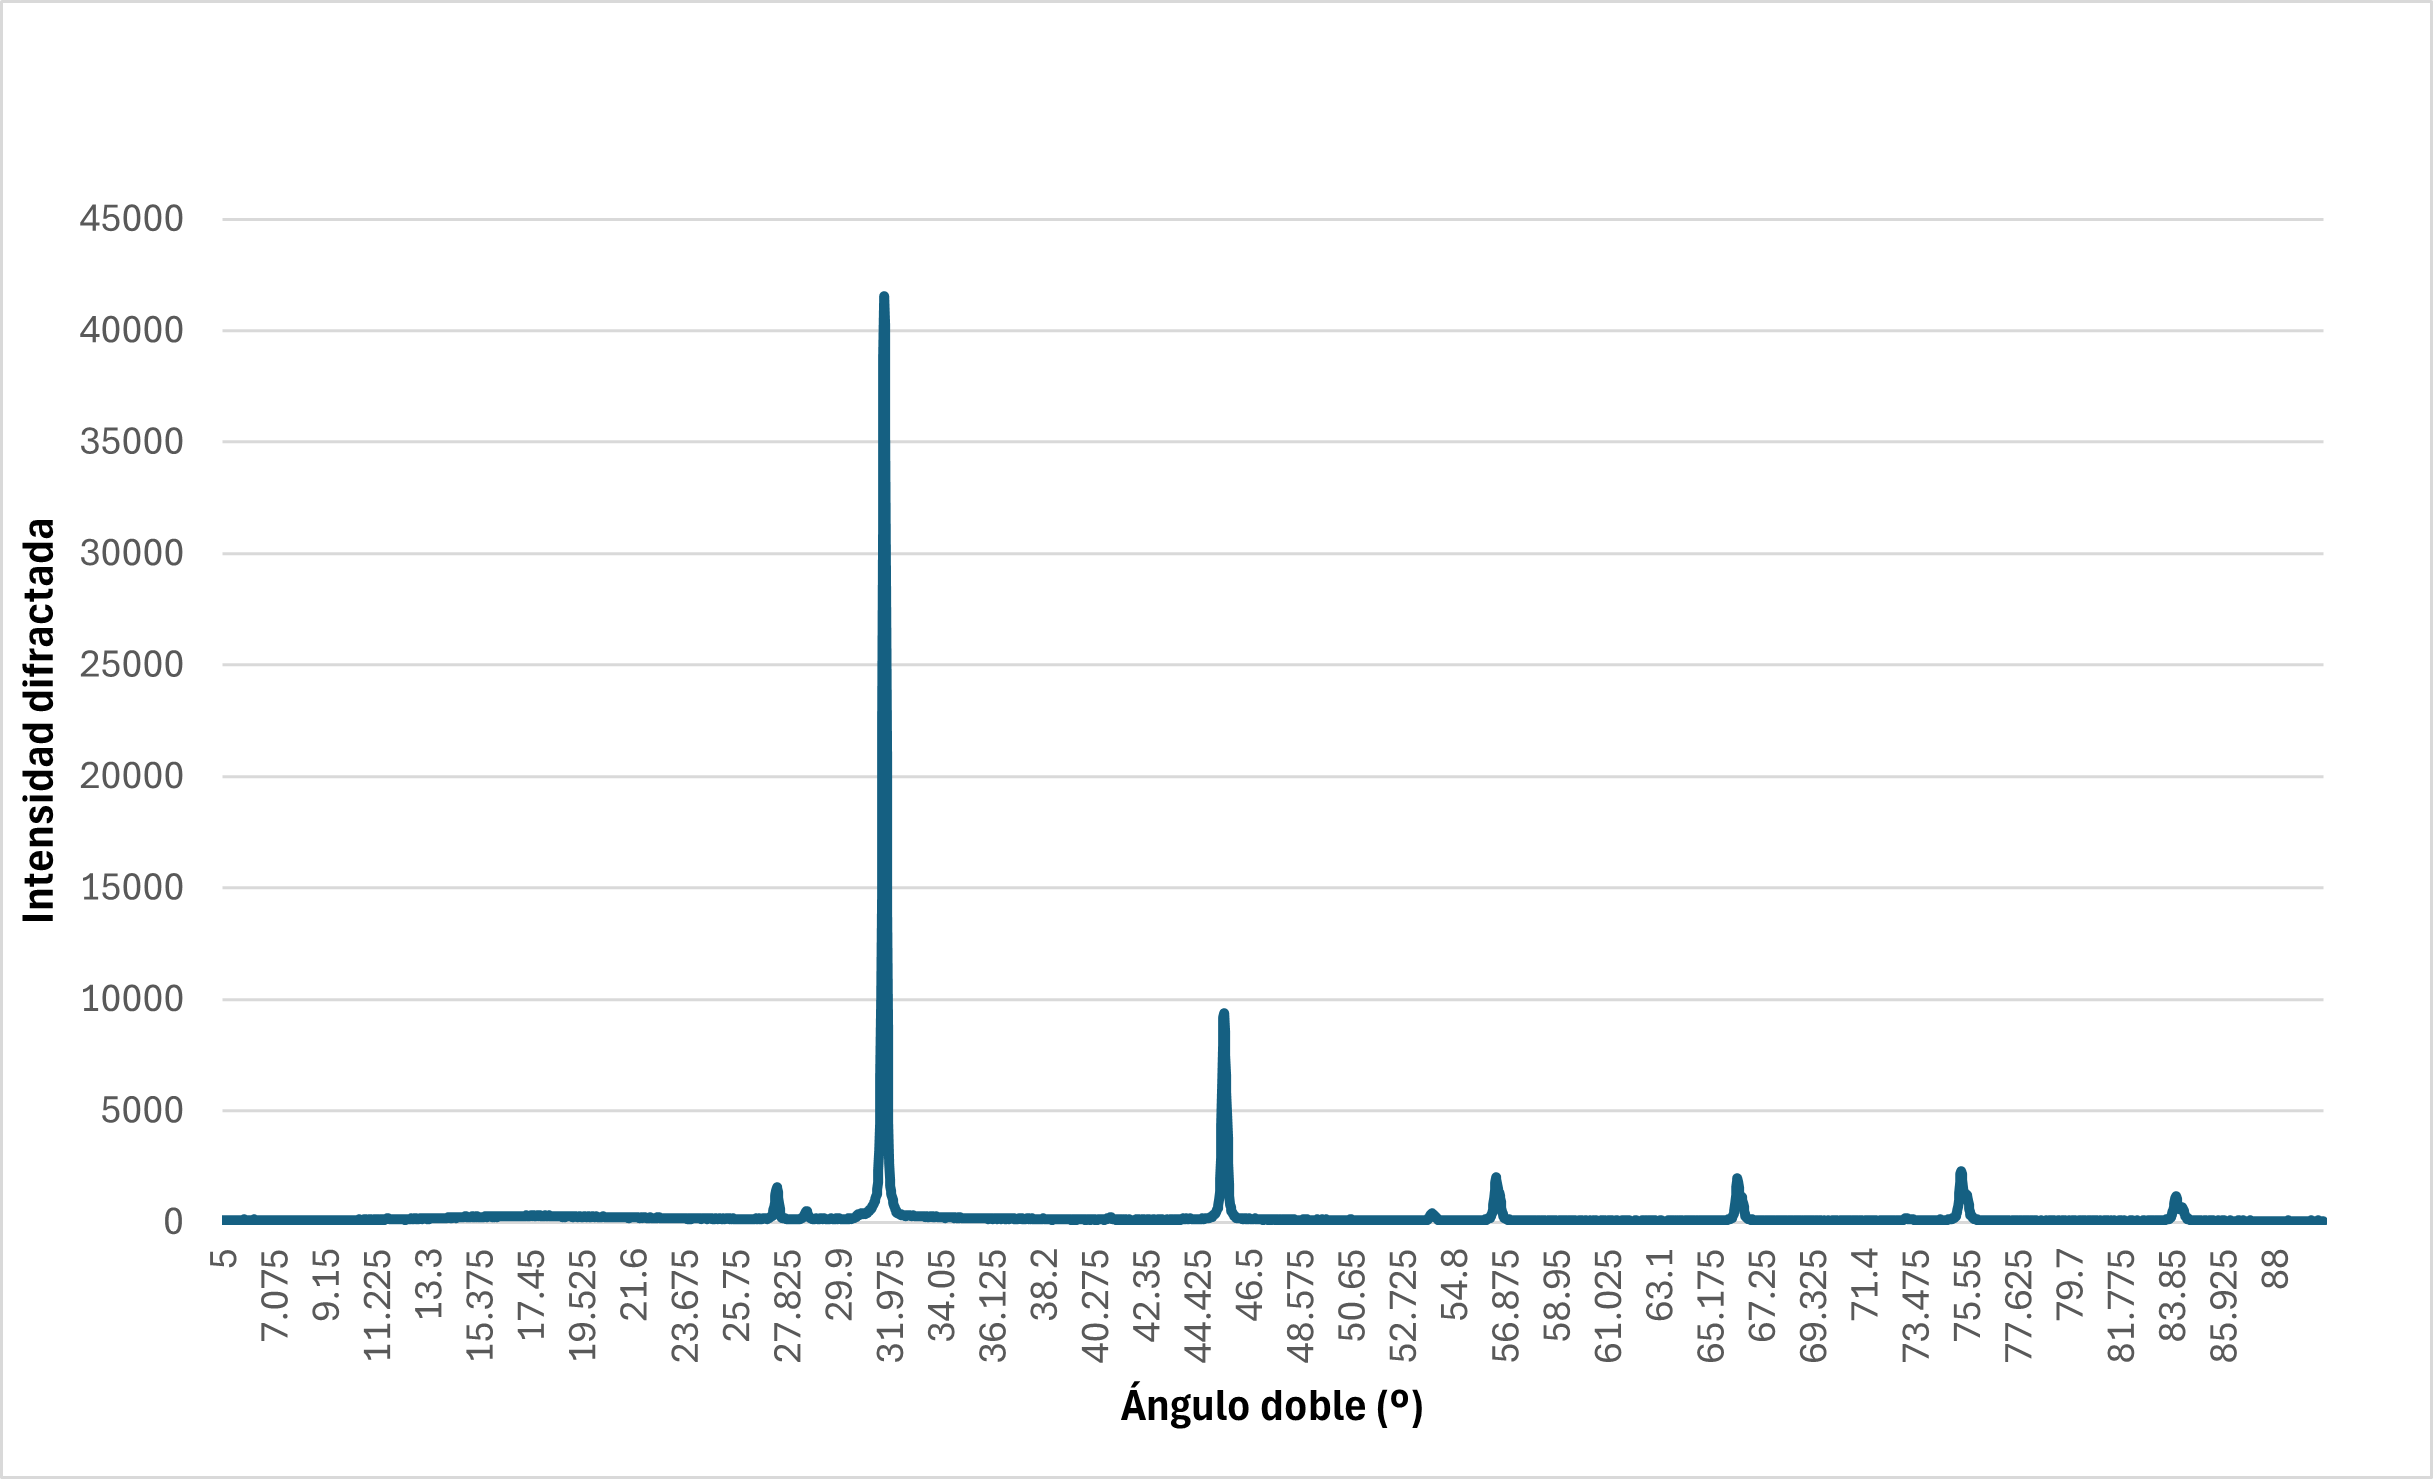
\includegraphics[max width=\linewidth]{DifNaCl.png}
        \end{center}
        \caption{Picos de difracción obtenidos para el cloruro de sodio.}
    \end{figure}
\end{frame}
\begin{frame}
    Usaremos intensidades relativas entre los dos picos de cada orden:
    \begin{equation}
        \frac{I_{(hkl)}^{max}}{I_{(hkl)}^{min}} = \left(\frac{f_{Na} + f_{Cl}}{f_{Na} - f_{Cl}}\right)^2
    \end{equation}
    \begin{table}
        \begin{center}
            \begin{tabular}{|c|c|c|c|}
                \hline
                n & 1 & 2 & 3 \\ \hline
                Ratio & $26.662$ & $41.224$ & $5.193$ \\ \hline
            \end{tabular}
        \end{center}
        \caption{Cociente entre intensidades para diversos órdenes de difracción.}
    \end{table}
    \begin{block}{Algunas observaciones}
        El cociente entre intensidades no es constante. El error puede deberse:
        \begin{itemize}
            \item El modelo de factor de forma constante, aunque bueno para encontrar las leyes de extinción, no es tan útil para luego determinar los factores.
            \item La difracción por rayos X no es una buena metodología para determinar los factores de forma.
        \end{itemize}
    \end{block}
\end{frame}
\begin{frame}{Radios atómicos}
    \subsection{Radios atómicos}
    Nuestro último objetivo será intentar calcular los radios atómicos del $Na^+$ y el $Cl^-$ en la red, usando el cálculo del parámetro de red. Supondremos que $R_{Na} > R_{Cl}$, puesto que la mayor electronegatividad del cloro, hará que la función de onda del electrón este menos extendida.
    \begin{figure}[h!]
        \begin{center}
            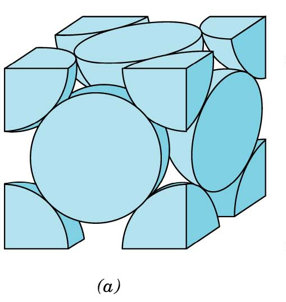
\includegraphics[max width=0.3\linewidth]{FCCDensity.png}
        \end{center}
        \caption{Imagen de la celda unidad de una red FCC en un modelo de esferas rígidas. Tomado de las diapositivas del tema 2 de la asignatura de Ciencia de los Materiales - prof. Joaquín Silvestre.}
    \end{figure}
\end{frame}
\begin{frame}
    Supondremos que el cloro no molesta, trataremos como si una red FCC sólo de $Na^+$ se tratase. De la imagen anterior podemos deducir que:
    $$
    4R_{Na} = a\sqrt{2} \implies
    $$
    \begin{equation}
        R_{Na} = 1.992 \pm 0.004 \, \text{\r{A}}
    \end{equation}
    Suponiendo que el cloro ocupe la posición central, ocupando todo el espacio restante que deja el sodio:
    $$
    2R_{Na} + 2R_{Cl} = a \implies
    $$
    \begin{equation}
        R_{Cl} = 0.825 \pm 0.007 \, \text{\r{A}}
    \end{equation}
    \begin{block}{Comparación de resultados}
        Los valores de referencia son $R_{Cl} = 0.79 \, \text{\r{A}}$ y $R_{Na} = 1.9 \, \text{\r{A}}$. Nuestros resultados no coinciden en error con estos resultados.
    \end{block}
\end{frame}
\begin{frame}{Conclusiones}
    \section{Conclusiones}
    \begin{block}{Conclusiones}
        \begin{itemize}
            \item La difracción de rayos X es muy útil para determinar el parámetro de red y las distancias interplanares con precisión.
            \item Una vez conocidas las reglas de extinción, nos permite comprobar rápidamente el tipo de estructura que presenta una muestra.
            \item La metodología experimental o el método que utilizamos para el cálculo, no parecen ser útiles para obtener los factores de forma.
            \item Al igual que con los factores de forma, necesitaríamos otra metodología u otro modelo teórico para determinar los radios atómicos, aunque en este caso, nos aproximamos mejor a los mismos.
        \end{itemize}
    \end{block}
    Para el cálculo de los factores de forma, se pueden usar otras técnicas, como difracción a bajas energías y ángulos \cite{PhysRevLett.21.1388} o radiación de frenado \cite{PhysRevB.44.9248}. El radio sí que podría aproximarse por rayos X, quizás con mejores medidas, o utilizando otra muestra para cada elemento.
\end{frame}
\begin{frame}[allowframebreaks]{Referencias}
    \section{Referencias}
    \printbibliography
\end{frame}
\end{document}